\def\nr{10. Aufgabenblatt}
\def\kopf{\\\hfill\normalsize\mdseries}
\documentclass[11pt,a4paper,fleqn]{scrartcl}
\usepackage{eurosym}
\usepackage{adjustbox,csquotes}
%\usepackage{a4kopka}
\usepackage{amsmath,amssymb,amsthm,amsfonts}
\usepackage[utf8]{inputenc}
\usepackage{algorithmic,algorithm}
\usepackage{graphics,graphicx}
\usepackage{pgfplots,tikz}
\usepackage{enumerate}
\usepackage[ngerman]{babel}
% \usepackage[software]{mymacros}
%\usepackage{matrix}
\usepackage{hyperref}
% \usepackage{caption}
\usepackage{caption, subcaption}

\floatname{algorithm}{Algorithmus}
\renewcommand{\algorithmicrequire}{\textbf{Input:}}
\renewcommand{\algorithmicensure}{\textbf{Output:}}

%\usepackage{enumitem} 
%\textheight25cm
\textheight23cm
\topmargin-15mm
\oddsidemargin-5mm    %  -10mm
\textwidth17cm    %   18.8cm
\footskip0pt
\thispagestyle{empty}
\parindent0mm
\parskip0ex
\parskip0ex

\makeatletter
\DeclareOldFontCommand{\rm}{\normalfont\rmfamily}{\mathrm}
\DeclareOldFontCommand{\sf}{\normalfont\sffamily}{\mathsf}
\DeclareOldFontCommand{\tt}{\normalfont\ttfamily}{\mathtt}
\DeclareOldFontCommand{\bf}{\normalfont\bfseries}{\mathbf}
\DeclareOldFontCommand{\it}{\normalfont\itshape}{\mathit}
\DeclareOldFontCommand{\sl}{\normalfont\slshape}{\@nomath\sl}
\DeclareOldFontCommand{\sc}{\normalfont\scshape}{\@nomath\sc}
\makeatother

% \newcommand{\cg}[1]{{\color{blue} #1}}
% \newcommand{\cb}[1]{{\color{green} #1}}
% \newcommand{\cred}[1]{{\color{red} #1}}
% \newcommand{\cc}[1]{{\color{cyan} #1}}
% \newcommand{\cm}[1]{{\color{magenta} #1}}

\newcommand{\Aufgabe}[2][]{\par\bigskip{\sf\bfseries Aufgabe #2#1:}}
%\hspace{3em}{\small(#2 point\ifthenelse{#2>1}{s}{})}}\par\smallskip}
%\newcommand\aufgabe[2][~]{\par\bigskip{\sf\bfseries Aufgabe #1
%    \hspace{3em} \ifthenelse{\equal{#2}{~}}{}{(#2)}}\par\smallskip}
\usepackage{mymacros}

\begin{document}
{\sf Universit\"at Hamburg \hfill Wintersemester 2020/21 \\ Fachbereich Mathematik \\ Dr. Matthias Voigt}
\begin{center}
\ifthenelse{\equal{\nr}{no}}{\Large\sf\bfseries \kopf}{\Large\sf\bfseries Optimierung f\"ur Studierende der Informatik -- \nr.~\kopf}
\end{center}

\renewcommand{\tilde}{\widetilde}
\renewcommand{\hat}{\widehat}
\newcommand{\ri}{\mathrm{i}}
\renewcommand{\H}{\mathsf{H}}
\newcommand{\T}{\mathsf{T}}


\subsection*{Präsenzaufgaben am 25./26.01.2021}

\Aufgabe[ (ein gieriger Approximationsalgorithmus)]{P1}
Beim Entwurf von Approximationsalgorithmen spielen neben LP-basierten Methoden auch \textit{Greedy-Verfahren} eine wichtige Rolle. Im Folgenden wird ein Beispiel betrachtet, das dies illustriert.

\medskip

Ein Schiff mit $n$ Containern $1,2,\ldots,n$ erreicht den Hafen. Die Abmessungen der Container spielen keine Rolle, es geht ums Gewicht: Container $i$ habe das Gewicht $w_i > 0$ ($i=1,\ldots,n$). Zum Weitertransport stehen Lastwagen bereit, von denen jeder einen oder mehrere Container aufnehmen kann. \textit{Einzige Restriktion}: Es gibt eine Gewichtsschranke $K$, die für jeden Laster gilt, d.h., kein Lastwagen darf Container von einem Gesamtgewicht größer $K$ aufnehmen. Die Schranke $K$ und auch die Gewichte $w_i$ sollen als ganzzahlig angenommen werden. Es gelte $K \geq w_i$ für $i=1,\ldots,n$. Zu minimieren ist die Anzahl der Lastwagen, die zum Weitertransport aller Container benötigt werden. (Anmerkung: Das beschriebene Problem ist ein NP-schweres Optimierungsproblem.)

\textit{Ein Greedy-Algorithmus}: Die Container werden in der Reihenfolge $1,2,\ldots, n$ verladen, wobei immer nur ein Lastwagen zur Zeit beladen wird. Immer, wenn der nächste Container nicht mehr aufgeladen werden kann (wegen Überschreitung von $K$), wird ein Lastwagen für \enquote{voll} erklärt und auf die Reise geschickt.

\medskip

Mit $m^\star$ sei das optimale Ergebnis bezeichnet, d.h., $m^\star$ ist die minimale Anzahl der benötigten Lastwagen. Das Ergebnis, das der Greedy-Algorithmus liefert, werde mit $m$ bezeichnet. 

\begin{enumerate}[a)]
% Aufgabe P-1a
\item Belegen Sie anhand eines Beispiels, dass der Greedy-Algorithmus nicht immer das bestmögliche Ergebnis liefert. Mit anderen Worten: $m > m^\star$ ist möglich.

% Aufgabe P-1b
\item \textbf{Behauptung}: Es gilt immer $m < 2m^\star$. (Dies bedeutet, dass unser Greedy-Algorithmus gar nicht so schlecht ist: Es handelt sich um einen \textit{2-Approximationsalgorithmus}.)

\smallskip

Zeigen Sie die Richtigkeit dieser Behauptung für den Fall, dass $m$ ungerade ist.

\textbf{Hinweis}: $L_i$ sei das Gewicht, das der Greedy-Algorithmus auf den $i$-ten Lastwagen packt ($i=1,\ldots,m$). Welche naheliegende Feststellung lässt sich für die Summe $L_1+L_2$ und die Schranke $K$ treffen?
\end{enumerate}

\Aufgabe[ (ein Approximationsalgorithmus für das Knotenüberdeckungsproblem)]{P2}
In Vorlesung 9 wurde ein 2-Approximationsalgorithmus für das Knoten\-über\-deckungs\-problem vorgestellt.
\begin{enumerate}[a)]
% Aufgabe P-2a
\item Beschreiben Sie kurz in eigenen Worten, worum es beim Knotenüberdeckungsproblem geht.
% Aufgabe P-2b
\item Beschreiben Sie kurz (ebenfalls in eigenen Worten), wie der erwähnte 2-Approximations\-al\-go\-rith\-mus funktioniert.
% Aufgabe P-2c
\item Begründen Sie kurz, weshalb für die vom Algorithmus gelieferte Knotenüberdeckung $U$ gilt: $|U| \leq 2c(G)$.
% Aufgabe P-2d
\item Was versteht man unter dem vollständig bipartiten Graphen $K_{n,n}$?
\end{enumerate}

\subsection*{Hausaufgaben bis zum 03.02.2021 (12:00 Uhr)}
\emph{Bitte reichen Sie Ihre Hausaufgaben in festen Zweier- oder Dreiergruppen bei Moodle ein. Bitte laden Sie ausschließlich \textbf{PDF-Dokumente} hoch, andernfalls können Ihre Hausaufgaben nicht korrigiert werden.}

\Aufgabe[ ($k$-Hitting-Sets, 5 Punkte)]{H1}
Es sei $k \geq 2$ eine fest gewählte ganze Zahl. Gegeben sei eine Menge $S$ und eine Kollektion $T_1,\ldots,T_m$ von $k$-elementigen Teilmengen von $S$. Es gelte also
\[
T_i \subseteq S \text{  und  } |T_i|=k \quad (i=1,\ldots,m).
\]

Eine Teilmenge $H \subseteq S$ wird ein \textit{Hitting-Set} genannt, falls alle Mengen $T_i$ von $H$ getroffen werden, d.h., falls $H \cap T_i \neq \emptyset$ für alle $i = 1,\ldots,m$ gilt. Gesucht ist ein Hitting-Set mit einer minimalen Anzahl von Elementen. Wir nennen das beschriebene Problem $k$-Hitting-Set-Problem. Das Problem lässt sich also wie folgt beschreiben:
\medskip
\begin{center}
\begin{minipage}{0.85\textwidth}
\textbf{$\mathbf{k}$-Hitting-Set-Problem:}

\medskip
\textbf{Eingabe}: eine Menge $S$ sowie eine Kollektion von $k$-elementigen Teilmengen von $S$.

\medskip
\textbf{Gesucht}: ein Hitting-Set mit einer minimalen Anzahl von Elementen.
\end{minipage}
\end{center}

\medskip
Man beachte: $k$ ist \textit{nicht} Teil der Eingabe, sondern eine \textit{Konstante}.


\begin{enumerate}[a)]
% Aufgabe H-2b (i)
\item Beschreiben Sie einen $3$-Approximationsalgorithmus für das $3$-Hitting-Set-Problem.

% Aufgabe H-2b (ii)
\item Weisen Sie nach, dass der von Ihnen unter a) vorgeschlagene Algorithmus tatsächlich ein $3$-Appro\-xima\-tions\-algorithmus ist.
\end{enumerate}

\textbf{Hinweis:} Denken Sie zunächst an den Spezialfall $k=2$. Sie kennen bereits einen 2-Approxi\-mations\-algorithmus für diesen Spezialfall aus Vorlesung~9.

\Aufgabe[ (Residualgraphen, 5 Punkte)]{H2}
Betrachten Sie folgendes Flussnetzwerk $N=(G,c,s,t)$ mit einem Fluss $f$ mit $w(f) = 20$:
\begin{center}
 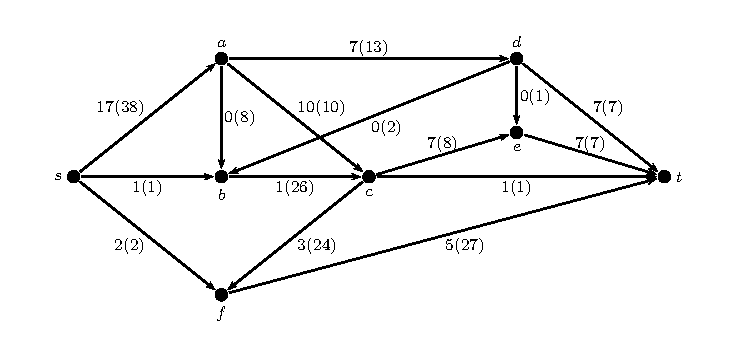
\includegraphics{fig10_1.pdf}
\end{center}

\begin{enumerate}[a)]
 \item Zeichnen Sie den Residualgraphen $G_f$ des oben abgebildeten Netzwerks. \pagebreak
 \item Führen Sie eine Iteration des Algorithmus von Edmonds und Karp auf dem in a) bestimmten Residualgraphen durch. Überlegen Sie sich dazu, wie die Markierungen aussehen müssen und schreiben Sie diese an die Knoten. 
 
 Verwenden Sie wie immer folgende Regel: Stehen mehrere Knoten zur Markierung zur Verfügung, so ist derjenige Knoten zu markieren, der zuerst im Alphabet kommt.
 
 \item Beschreiben Sie, wie der Residualgraph am Ende einer jeden Iteration aktualisiert werden muss.
\end{enumerate}

\end{document}
